\section{Inferencia Basada en Verosimilitud}


\subsection{Caso Uniparamétrico}

Toda información acerca de $\theta$ que los datos nos proporcionan está en la función de verosimilitud.

\textbf{\textit{Definición: }} Sean $X_1, \dots, X_n$ v.a.i.i.d. Se define como función de verosimilitud a

\[
    L(\theta; X_1,\dots,X_n) =
    \begin{cases}
        P_\theta(X_1,\dots,X_n)=\prod_{i=1}^{n}P_\theta(X_i=x_i) & \text{Caso discreto} \\
        f(X_1,\dots,X_n; \theta)=\prod_{i=1}^{n}f(x_i; \theta)   & \text{Caso continuo}
    \end{cases}
\]

$L(\theta; X_1,\dots,X_n)$ es una función de $\theta$ proporcional a la probabilidad de observar que $(X_1,\dots,X_n)=(x_1,\dots,x_n)$ cuando $\theta$ es el verdadero valor del parámetro. Así, un valor del parámetro será más o menos verosimil cuanto mayor o menor sea esa verosimilitud.

Consideremos las siguientes condiciones:

\begin{enumerate}
    \item El parámetro $\theta$ es identificable, es decir, que $\theta \neq \theta' \implies P_\theta \neq P_{\theta'}$
    \item Las distribuciones $P_\theta$ donde $\theta \in \Theta$ tienen el mismo soporte $\{x:f(x,\theta) > 0\}$ y no depende de $\theta$
\end{enumerate}

\textbf{\textit{Resultado: }} Sean $X_1,\dots,X_n$ v.a.i.i.d. con $f(X;\theta)$. Entonces si $\theta_0$ es el verdadero valor del parámetro

\[
    P_\theta(L(\theta_0;X_1,\dots,X_n)>L(\theta;X_1,\dots,X_n))\xrightarrow{n\to\infty}1
\]

\begin{proofs}
    Sea
    \[
        \left\{x:L(\theta_0;X_1,\dots,X_n)>L(\theta;X_1,\dots,X_n)\right\}=\left\{x:\prod_{i=1}^{n}\frac{f(x_i;\theta)}{f(x_i;\theta_0)}<1\right\}
    \]
    \[
        \left\{x:\frac{1}{n}\sum_{i=1}^{n}\log{\frac{f(x_i;\theta)}{f(x_i;\theta_0)}}<0\right\}
    \]
    Tenemos que
    \[
        \frac{1}{n}\sum_{i=1}^{n}\log{\frac{f(x_i;\theta)}{f(x_i;\theta_0)}} \overset{P}{\to}E_{\theta_0}=\left(\log{\frac{f(x_i;\theta)}{f(x_i;\theta_0)}}\right)
    \]
    Aplicando la desigualdad de Jensen para funciones convexas: $f(E(X)) \leq E(f(X))$ donde $-\log$ es convexa
    \[
        E_{\theta_0}\left(-\log{\frac{f(x_i;\theta)}{f(x_i;\theta_0)}}\right) \geq -\log{E_{\theta_0}\left(\frac{f(x_i;\theta)}{f(x_i;\theta_0)}\right)} \implies
    \]
    \[
        \implies E_{\theta_0}\left(\log{\frac{f(x_i;\theta)}{f(x_i;\theta_0)}}\right) \leq \log{E_{\theta_0}\left(\frac{f(x_i;\theta)}{f(x_i;\theta_0)}\right)}
    \]
    \[
        \log{E_{\theta_0}\left(\frac{f(x_i;\theta)}{f(x_i;\theta_0)}\right)}=\log\int\frac{f(x_i;\theta)}{f(x_i;\theta_0)}f(x_i;\theta_0)dx=\log\int f(x_i;\theta_0)dx=\log(1)=0
    \]
    probamos que $\frac{1}{n}\sum_{i=1}^{n}\log{\frac{f(x_i;\theta)}{f(x_i;\theta_0)}}$ converge a una cantidad negativa
\end{proofs}

\subsubsection{Estimación por Máxima Verosimilitud}

El estadistico EMV es el valor en el que se alcanza el máximo de la verosimilitud o así mismo, puesto que la transformación logaritmica es monótona y creciente, de la log verosimilitud definida como $l(\theta;X_1,\dots,X_n)=\log L(\theta;X_1,\dots,X_n)$. \\

\textbf{\textit{Definición: }} $\widehat{\theta}(x)$ será EMV de $\theta$ si

\[
    \widehat{\theta}(x) = \underset{\theta \in \Theta}{argmax}(l(\theta;X_1,\dots,X_n))
\]

\begin{figure}[h!]
    \begin{minipage}{0.48\textwidth}
        \centering

        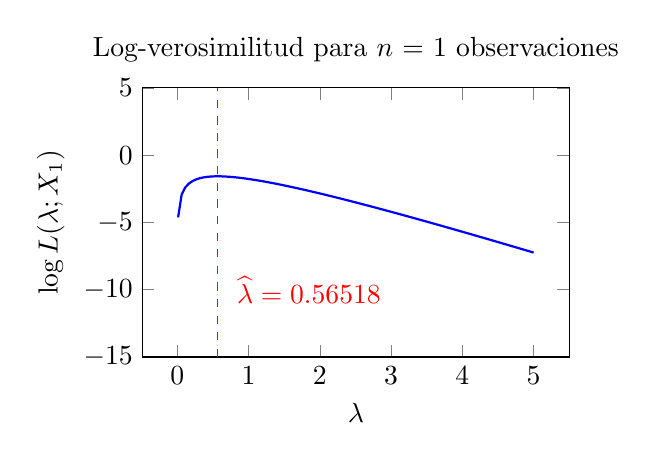
\begin{tikzpicture}
            \begin{axis}[
                    domain=0.01:5,
                    samples=100,
                    ymin=-15, ymax=5,
                    xlabel={$\lambda$},
                    ylabel={$\log L(\lambda; X_1)$},
                    title={Log-verosimilitud para $n$ = 1 observaciones},
                    width=7cm, height=5cm
                ]
                \addplot[thick,blue] {ln(x) - x*1.769362};
                \addplot[red, dashed] coordinates {(0.56518, -15) (0.56518, 5)};.
                \node at (axis cs: 0.7, -10) [anchor=west, red] {$\widehat{\lambda} = 0.56518$};
            \end{axis}
        \end{tikzpicture}

    \end{minipage}
    \hfill
    \begin{minipage}{0.48\textwidth}
        \centering

        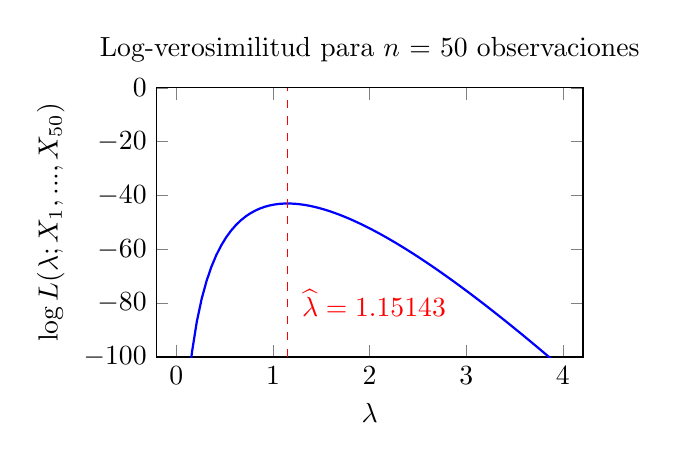
\begin{tikzpicture}
            \begin{axis}[
                domain=0.01:5,
                samples=100,
                ymin=-100, ymax=0,
                xlabel={$\lambda$},
                ylabel={$\log L(\lambda; X_1,...,X_{50})$},
                title={Log-verosimilitud para $n$ = 50 observaciones},
                width=7cm, height=5cm
                ]
                \addplot[thick,blue] {50*ln(x) - x*43.42423};
                \addplot[red, dashed] coordinates {(1.15143, -100) (1.15143, 0)};
                \node at (axis cs: 1.2, -80) [anchor=west, red] {$\widehat{\lambda} = 1.15143$};
            \end{axis}
        \end{tikzpicture}

    \end{minipage}

    \begin{center}

        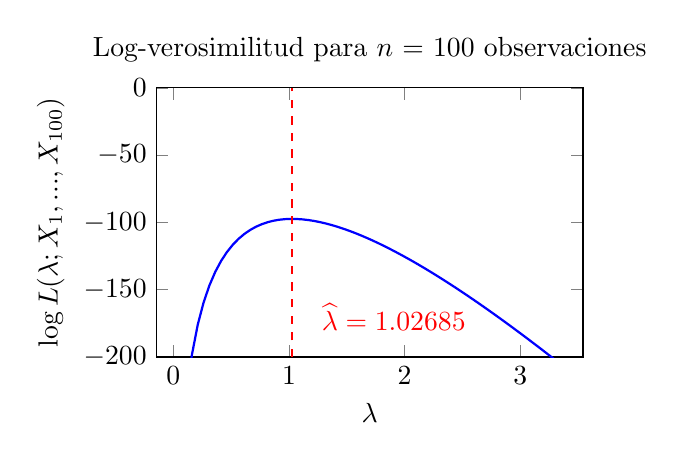
\begin{tikzpicture}
            \begin{axis}[
                domain=0.01:5,
                samples=100,
                ymin=-200, ymax=0,
                xlabel={$\lambda$},
                ylabel={$\log L(\lambda; X_1,...,X_{100})$},
                title={Log-verosimilitud para $n$ = 100 observaciones},
                width=7cm, height=5cm
                ]
                \addplot[thick,blue] {100*ln(x) - x*97.38531};
                \addplot[red, dashed] coordinates {(1.02685, -200) (1.02685, 0)};
                \node at (axis cs: 1.2, -170) [anchor=west, red] {$\widehat{\lambda} = 1.02685$};
            \end{axis}
        \end{tikzpicture}
        \caption{Podemos observar como el EMV aproxima el verdadero valor de $\lambda$ en función de la cantidad de observaciones (en este caso $\exp(\lambda)$ donde $\lambda = 1$)}

    \end{center}
    \label{fig:exp-log-ver}
\end{figure}

En la siguiente página se mostrará un ejemplo de como calcular el estimador máximo verosimil de una distribución Bernoulli de parametro $\theta$.

\newpage

\begin{exercise}
    Sean $X_1,\dots,X_n$ v.a.i.i.d. donde $X_i \thicksim B(\theta)$ para $\theta \in (0,1)$. Sea la función de distribución Bernoulli $P_\theta(X=x)=\theta^x(1-\theta)^{1-x}$. Estimar $\theta$ mediante máxima verosimilitud. \\
    Calculamos la verosimilitud como
    \[
        L(\theta;X) \propto \prod_{i=1}^{n}\theta^x(1-\theta)^{1-x}=\theta^{\sum_{i=1}^{n}x_i}(1-\theta)^{n-\sum_{i=1}^{n}x_i}
    \]
    y la log verosimilitud
    \[
        l(\theta; X_1,\dots,X_n)=\sum_{i=1}^{n}x_i\log\theta + (n-\sum_{i=1}^{n}x_i)\log(1-\theta)
    \]
    Encontraremos un máximo en donde se cumpla que $\frac{\partial}{\partial\theta}l(\theta;X_1,\dots,X_n)=0$
    \[
        \frac{\partial}{\partial\theta}l(\theta;X_1,\dots,X_n) = \frac{\sum_{i=1}^{n}x_i}{\theta}-\frac{n-\sum_{i=1}^{n}x_i}{(1-\theta)} \implies
    \]
    \[
        \implies \sum_{i=1}^{n}x_i(1-\theta)=(n-\sum_{i=1}^{n}x_i)\theta \implies \theta=\frac{\sum_{i=1}^{n}x_i}{n}=\overline{X}
    \]
    Por tanto concluimos que el EMV de $\theta$ es $\widehat{\theta}=\overline{X}$.
\end{exercise}

\vspace{30pt}

Hilando con la figura \ref{fig:exp-log-ver} donde vemos representada la log verosimilitud de una exponencial, se pondrá como ejemplo también el cálculo del EMV de una distribución exponencial censurada negativa de parámetro $\lambda$.

\textbf{\textit{Definición: }} Sean $X_1, \dots, X_n$ v.a.i.i.d. que siguen una distribución exponencial. Se considera como censura a la derecha cuando se desconoce el tiempo exacto de fallo para $k$ observaciones, pero si se sabe que ocurrió después de un tiempo $t_0$. Es decir, que para $k$ observaciones solo sabemos que $x_i > t_0$.

\vspace{30pt}

Se resolverá el ejercicio en la siguiente página...

\newpage

\begin{exercise}
    Sean $X_1, \dots, X_n$ v.a.i.i.d. donde $X_i$ sigue una exponencial negativa censurada a la derecha de parámetro $\lambda$. Sea la función de distribución exponencial $f(x;\lambda)=\lambda e^{-\lambda x}$. Estimar $\lambda$ mediante máxima verosimilitud. \\
    La función de verosimilitud tendrá dos tipos de datos, los que se obtienen de la exponencial ($f_\lambda(x;\lambda)$) y los $k$ censurados ($P(X_i>t_0)$). \\
    Entonces la función de verosimilitud queda de la siguiente forma:
    \[
        L(\lambda; x_1,\dots,x_n)=\left(\prod_{i=1}^{k}\lambda e^{-\lambda x_i}\right)\left(\prod_{i=k+1}^{n}P(X_i>t_0)\right)
    \]
    Sabemos que
    \[
        P(X_i>t_0)=\int_{t_0}^\infty \lambda e^{-\lambda x}dx = e^{-\lambda t_0}
    \]
    Por lo tanto
    \[
        L(\lambda;x_1,\dots,x_n)=\lambda^k e^{\lambda \sum_{i=1}^{k}x_i}e^{-\lambda(n-k)t_0}
    \]
    Y la log verosimilitud queda
    \[
        l(\lambda;x_1,\dots,x_n)=k\log\lambda-\lambda\left(\sum_{i=1}^{k}x_i + (n-k)t_0\right)
    \]
    Que encontrará máximo en $\widehat{\lambda} = \frac{k}{\sum_{i=1}^{k}+(n-k)t_0}$
\end{exercise}

Como último ejemplo se hará lo mismo con la distribución Poisson

\begin{exercise}
    Sean $X_1, \dots, X_n$ v.a.i.i.d. donde $X_i$ sigue una Poisson de parámetro $\lambda$. Sea la función de distribución Poisson $P_\lambda(X=x)=\frac{e^{-\lambda}\lambda^x}{x!}$. Estimar $\lambda$ mediante máxima verosimilitud y comprobar si el estimador es CAN y AE. \\
    La verosimilitud quedará como
    \[
        L(\lambda;x_1,\dots,x_n)=\prod_{i=1}^{n}\frac{e^{-\lambda}\lambda^{x_i}}{{x_i}!}
    \]
    siendo la log verosimilitud
    \[
        l(\lambda; x_1,\dots,x_n)=-n\lambda+\sum_{i=1}^{n}x_i\log\lambda
    \]
    Que encontrará máximo en $\widehat{\lambda}=\overline{X}$ \\
    Haciendo uso de este último resultado, es fácil comprobar que $\widehat{\lambda}$ es CAN y AE pues
    \[
        \sqrt{n}(\widehat{\lambda}-\lambda)=\sqrt{n}(\overline{X}-\lambda) \overset{L}{\to}N(0,\frac{1}{I_1(\lambda)})
    \]
    \[
        I_1(\lambda)=\frac{1}{\lambda} \implies \sqrt{n}(\overline{X}-\lambda)\overset{L}{\to}N(0,\lambda)\square
    \]
\end{exercise}

\newpage

Como generalización del anterior resultado se enuncia el siguiente teorema

\begin{theorem}
    Sean $X_1,\dots,X_n$ v.a.i.i.d. con función de densidad $f(x;\theta)$ donde $\theta \in \Theta$ que verifica CRCR y además que
    \[
        \exists \frac{\partial^3}{\partial \theta^3}\log f(x;\theta) \quad \text{y} \quad \left|\frac{\partial^3}{\partial \theta^3}\log f(x;\theta)\right| \leq M(X); \quad E(M(X))<\infty
    \]
    Entonces el EMV de $\theta$ es CAN y AE. Es decir
    \[
        \sqrt{n}(\widehat{\theta}(X)-\theta)\overset{L}{\to}N(0,\frac{1}{I_1(\theta)})
    \]
\end{theorem}

Pongamos un ejemplo

\begin{exercise}
    Sean $X_1, \dots, X_n$ v.a.i.i.d. donde $X_i$ sigue una Normal de parámetros $(0,\sigma^2)$ donde $\sigma^2=\theta$. Sea la función de distribución Normal $f(x;\theta)=\frac{1}{\sqrt{(2\pi\theta)}}e^{\frac{-x^2}{2\theta}}$. Entonces
    \[
        L(\theta;x_1,\dots,x_n)=\frac{1}{\sqrt{\theta}}e^{\frac{-\sum_{i=1}^{n}x^2_i}{2\theta}} \implies l(\theta;x_1,\dots,x_n)=-\frac{n}{2}\log\theta - \frac{\sum_{i=1}^{n}x^2_i}{2\theta}
    \]
    Que encontrará máximo en $\widehat{\theta}=\frac{\sum_{i=1}^{n}x^2_i}{n}$. Entonces
    \[
        \sqrt{n}\left(\frac{\sum_{i=1}^{n}x^2_i}{n}-\theta\right)\overset{L}{\to}N\left(0,\frac{1}{I_1(\theta)}\right)
    \]
    \[
        I_1(\theta)=Var\left(-\frac{n}{2\theta}+\frac{\sum_{i=1}^{n}x^2_i}{2\theta^2}\right)=\frac{n}{2\theta^2}
    \]
    por tanto
    \[
        \sqrt{n}\left(\frac{\sum_{i=1}^{n}x^2_i}{n}-\theta\right) \overset{L}{\to}N(0,2\theta^2) = N(0,2\sigma^4)
    \]
\end{exercise}

Se podría hacer también para una Normal $N(0,\sigma)$ donde $\widehat{\theta}=\sqrt{\frac{\sum_{i=1}^{n}x^2_i}{n}}$ que es el EMV para $\sigma$ en modelos $N(0,\sigma)$
Queda como ejercicio para el lector comprobar si

\[
    \sqrt{n}\left(\sqrt{\frac{\sum_{i=1}^{n}x^2_i}{n}}-\sigma\right)\overset{L}{\to}N\left(0,\frac{1}{I_1(\sigma)}\right)
\]
\newpage
\subsubsection{Intervalos de confianza y contrastes de hipótesis uniparamétricos}

Ya hemos visto como estimar el EMV en el caso uniparamétrico. Ahora vamos a ver como se hacen los intervalos de confianza y los contrastes de hipótesis.

\hspace{-1cm}\noindent\begin{tabular}{r}
    \textbf{Ejemplo}  \\ \hline \ \\
\end{tabular}\\
Sean $X_1\dots X_n\sim B(\theta)$ con $0<\theta < 1$, $f(x,\theta)=\theta^x(1-\theta)^{1-x}$, $E(X)=\theta$\ y\ \ $Var(X)=\theta(1-\theta)$

Recordemos que el EMV para $X\sim B(\theta)$ es $\widehat\theta_n=\overline{X}$
$$I_1(\theta)=-E\Big(\frac{\partial^2}{\partial\theta^2}ln(f(x,\theta))\Big)=\frac{\theta^2-2\theta^2+\theta}{\theta^2(1-\theta)^2}=\frac{1}{\theta(1-\theta)}$$

Por lo tanto: 
$$\sqrt{n}(\overline{X}-\theta)\overset{\mathcal{L}}{\longrightarrow}N\big(0,\theta(1-\theta)\big)$$

Usando esta distribución asintótica podemos construir \textbf{intervalos de confianza} para $\theta$.
$$P_\theta\Bigg(\underbrace{\frac{\sqrt{n}|\overline{X}-\theta|}{\sqrt{\theta(1-\theta)}}}_{N(0,1)}<\zeta_{1-\frac{\alpha}{2}}\Bigg)=1-\alpha$$

Buscamos el cuantil $\zeta_{1-\frac{\alpha}{2}}$ que hace que la probabilidad sea $1-\alpha$
$$P_\theta\Bigg(-\zeta_{1-\frac{\alpha}{2}}<\frac{\sqrt{n}(\overline{X}-\theta)}{\sqrt{\theta(1-\theta)}}<\zeta_{1-\frac{\alpha}{2}}\Bigg)=1-\alpha$$

Utilizamos la información de Fischer $I_n(\theta)=\frac{n}{\theta(1-\theta)}$ para depejar $\theta$
$$P_\theta\Bigg(-\zeta_{1-\frac{\alpha}{2}}<\frac{(\overline{X}-\theta)}{\sqrt{\frac{1}{I_n(\theta)}}}<\zeta_{1-\frac{\alpha}{2}}\Bigg)=1-\alpha$$
$$P_\theta\Bigg(\overline{X}-\zeta_{1-\frac{\alpha}{2}}\sqrt{\frac{1}{I_n(\theta)}}<\theta<\overline{X}+\zeta_{1-\frac{\alpha}{2}}\sqrt{\frac{1}{I_n(\theta)}}\Bigg)=1-\alpha$$

    \textit{\textbf{Definición:}} La \textbf{Información de Fischer observada }se traduce en sustituir la información de Fischer esperada por su EMV. Como $\widehat\theta_n$ es CAN para $\theta$, se tiene que
    $$If_{obs}\overset{p}{\longrightarrow}If_{esp}$$

\noindent En nuestro caso particular consiste en reemplazar $I_n(\theta)=\frac{n}{\theta(1-\theta)}$ por $I_n(\widehat\theta)=\frac{n}{\overline{X}(1-\overline{X})}$, luego:
$$P_\theta\Bigg(\overline{X}-\zeta_{1-\frac{\alpha}{2}}\sqrt{\frac{\overline{X}(1-\overline{X})}{n}}<\theta<\overline{X}+\zeta_{1-\frac{\alpha}{2}}\sqrt{\frac{\overline{X}(1-\overline{X})}{n}}\Bigg)=1-\alpha$$

Este tipo de inferencia basada en la verosimilitud se llama \textbf{inferencia de Wald}.\\

Para los contrastes de hipótesis vamos a definir tres estadísticos que nos sirven para hacer inferencia basada en la verosimilitud.
\begin{enumerate}
    \item \textbf{Estadístico de Razón de Verosimilitud}\\\ \\
    Definamos $\lambda (X)$
    $$\lambda (X)=\lambda (X_1,\dots ,X_n)=\Lambda (X)=\frac{L(\theta_0, X_1,\dots,X_n)}{\underset{\theta}{sup}\ L(\theta,X_1,\dots,X_n)}=\frac{L(\theta_0, X_1,\dots,X_n)}{L(\widehat\theta_n, X_1,\dots,X_n)}\in [0,1]$$
    $H_0$ se rechazará para valores bajos del estadístico. 
    Ahora vamos a hallar la \textbf{región crítica del test} $\lambda (X)<k$. Para hacerlo más sencillo, se puede escribir con la log-verosimilitud:
    $$Q_L=-2ln(\lambda (X))=-2\big(ln(L(\widehat\theta_n,X_1\dots,X_n))-ln(L(\theta_0,X_1\dots,X_n))\big)$$
    En este caso, se rechazará $H_0$ para valores grandes. La región crítica del test será $Q_L>C$. 
    Necesitamos conocer la distribución asintótica de $Q_L$, algo que veremos más adelante.

    \item \textbf{Estadístico de Wald}\\\ \\
    Bajo las condiciones de regularidad de Cramer-Rao podemos escribir $ln(L(\theta_0,X))$ como \textbf{desarrollo de Taylor} en torno a $\widehat\theta_n$ como:
    $$ln(L(\theta_0,X))\approx ln(L(\widehat\theta_n,X))+(\theta-\widehat\theta_n)\overbrace{\frac{\partial}{\partial\theta}ln(L(\widehat\theta_n,X))}^{0}+\frac{(\theta-\widehat\theta_n)^2}{2}\frac{\partial^2}{\partial\theta^2}ln(L(\widehat\theta_n,X))$$
    Recordemos que $\widehat\theta_n$ es el EMV, y por tanto el valor de su primera derivada es nula, pero el valor de su segunda derivada no tiene por qué serlo.
Ahora:
    $$Q_L=-2\big(ln(L(\widehat\theta_n,X))-ln(L(\theta_0,X))\big)=-2(ln(L(\theta_0,X))+\frac{(\theta-\widehat\theta_n)^2}{2}\frac{\partial^2}{\partial\theta^2}ln(L(\widehat\theta_n,X))-ln(L(\theta_0,X)))=$$
    $$=-2\Big(\frac{(\theta-\widehat\theta_n)^2}{2}\frac{\partial^2}{\partial\theta^2}ln(L(\widehat\theta_n,X))\Big)=(\theta-\widehat\theta_n)^2\Big(\underbrace{-\frac{\partial^2}{\partial\theta^2}ln(L(\widehat\theta_n,X))}_{\text{I. de Fischer observada}}\Big)=$$
    $$=(\theta-\widehat\theta_n)^2I_n(\theta)=\frac{n(\theta-\widehat\theta_n)^2}{Var(\widehat\theta_n)}=Q_W\longleftarrow\text{ \textbf{Estadístico de Wald}}$$
    $Q_L$ y $Q_W$ son asintóticamente equivalentes.

    \item \textbf{Estadístico de Rao}\\\ \\
    $$Q_R=R=\frac{\left(\overbrace{\frac{\partial}{\partial\theta}ln(L(\theta_0,X))}^{\text{Score}}\right)^2}{I_n(\theta)}$$
    Habíamos visto que 
    $$ln(L(\theta_0,X))\approx ln(L(\widehat\theta_n,X))+\frac{(\theta-\widehat\theta_n)^2}{2}I_n(\theta)$$
    Ahora vamos a calcular el desarrollo de Taylor para la función score en un entorno de $\widehat\theta_n$
    $$S(\theta_0)\approx \underbrace{S(\widehat\theta_n)}_{0}+(\theta_0-\widehat\theta_n)\frac{\partial^2}{\partial\theta^2}ln(L(\widehat\theta_n,X))$$
    \textit{(A partir de este punto el profesor hace una demostración que no es correcta, por lo que he preferido no incluirla, aunque las conclusiones que hay a continuación sí son validas)}\\\ \\
    Este resultado demuestra que $Q_R$ es asintóticamente equivalente a $Q_W$ y $Q_L$. 
\end{enumerate}

Los tres estadísticos rechazarán $H_0$ para valores grandes. Para ver qué distribución siguen, usamos $Q_W$.\\
Sabemos que un EMV es CAN y AE, por lo que:
$$\sqrt{n}(\widehat\theta_n-\theta)\overset{\mathcal{L}}{\longrightarrow}N\Big(0,\frac{1}{I_1(\theta)}\Big)\text{ y }\frac{\sqrt{n}(\widehat\theta_n-\theta)}{\sqrt{\frac{1}{I_1(\theta)}}}\overset{\mathcal{L}}{\longrightarrow}N(0,1)$$

$Q_W$ es $\displaystyle\frac{\sqrt{n}(\widehat\theta_n-\theta)}{\sqrt{\frac{1}{I_1(\theta)}}}$ al cuadrado, por lo que, despejando, se obtiene que:
$$n(\theta-\widehat\theta_n)^2I_1(\theta)\overset{\mathcal{L}}{\longrightarrow}\chi^2_1$$
En este punto es conveniente recordar que si una variable $Z\sim N(0,1)$ su cuadrado $Z^2\sim \chi^2_1$

Las distribuciones exactas de $Q_L$, $Q_W$ y $Q_R$ son diferentes, pero como las tres son \textbf{asintóticamente equivalentes}, tenderán a seguir una distribución $\chi^2_1$. 
Por tanto, para determinar el valor de la región crítica solo habría que calcular el siguiente percentil:
$$P_{\theta}(Q_i>c)\approx 1-\alpha\Longrightarrow  c=\chi^2_{1,1-\alpha}$$

\subsection{Caso multiparamétrico}

Situacion:
\(
X_1,\dots,X_n \quad i.i.d. \quad P_\theta,\theta \in \Theta \subseteq \mathbb{R}^s \)  

El parámetro s-dimensional es
\(
\theta = (\theta_1,\dots,\theta_s), \quad s \geq 1 \)
 con familia de densidad 

 \(
 \{ f(x,\theta),\theta_0 \in \Theta\}
\)

Igualmente podemos escribir

\begin{itemize}
    \item Función de verosimilitud: $L(\theta,X_1,\dots,X_n)=\prod^{n}_{i=1} f(x_i,\theta)$
    \item Función de log-verosimilitud: $l(\theta,X_1,\dots,X_n)=\sum^{n}_{i=1} \log f(x_i,\theta)$
    \item Vector/función score: $$S(\theta,X_1,\dots,X_n)=S(X,\theta)=\frac{d}{d \theta} \log L(\theta,X)
    = \left(\frac{d}{d \theta} \log L(\theta_1,X),\dots,\frac{d}{d \theta} \log L(\theta,X)\right)$$
\end{itemize}

Ahora nos preguntamos, ¿cual es la cantidad de información de Fisher que tendremos en el caso multiparamétrico?.
Para averiguarlo recurrrimos a la matriz Hessiana, que recordamos que es la matriz s x s de las derivadas parciales de segundo orden

\[
I_{ij}(\theta)=E_\theta\left(-\frac{d^2}{d \theta_i d \theta_j} log L(\theta,X)\right)
=E\left(\frac{d}{d \theta_i} log L(\theta,X),\frac{d}{d \theta_j} log L(\theta,X)\right)
\]
\[
H(\theta,X)=\left\{ \frac{d^2}{d \theta_i d \theta_j}log L(\theta,X) \right\}^s 
=
\begin{pmatrix}
    \frac{d^2}{d \theta_1^2}log L(\theta,X) & \dots & \frac{d^2}{d \theta_1 d \theta_s}log L(\theta,X) \\
    \vdots & \ddots & \vdots \\
    \frac{d^2}{d \theta_s d \theta_1}log L(\theta,X) & \dots & \frac{d^2}{d \theta_s^2}log L(\theta,X)
\end{pmatrix}
\]

Sabiendo esto, $I(\theta)$,matriz de información esperada(que recordemos que es la matriz de covarianzas del vectir score) será:
\[
I(\theta) = E_\theta(-H(\theta,X))
\]
Además de esto tendremos tambíen la matriz de información de Fisher observada

\subsubsection{EMV en el caso multiparamétrico}

$\widehat{\theta}=\widehat{\theta_n}=(\widehat{\theta_1},\dots,\widehat{\theta_s})'$ es el EMV para $\theta=(\theta_1,\dots,\theta_s)$
si es la solución al siguiente sistema de ecuaciones:

\[
\begin{matrix}
    \frac{d}{d \theta_1} log L(\theta,X)=0 \\
    \dots \\
    \frac{d}{d \theta_s} log L(\theta,X)=0
\end{matrix}
\]

Estas ecuaciones son las denominadas \textbf{ecuaciones de verosimilitud}.

\subsubsection*{Propiedades asintóticas del EMV multiparamétrico}

En la situación $X_1,\dots,X_n$ i.i.d. $P_\theta, \theta \in \Theta \subseteq \mathbb{R}^s s\geq1$
y bajo las siguientes condiciones de regularidad:

\begin{enumerate}
    \item $\Theta$ es un intervalo de $\mathbb{R}^s$
    \item El soporte de f no depende de $\theta$. $\{x:f(x,\theta)>0\}$ no depende de $\theta$.
    \item $\frac{d}{d \theta_j} f(x,\theta)$ existe y es finita $\forall j=1,\dots,s \quad \theta \in \Theta$
    \item La matriz de información de Fisher (IF($\theta$)) es definida positiva \[ (si \quad \forall X \neq A, \quad X^T \cdot A \cdot X >0) \]
    \item $f(x,\theta) \,dx$ se puede derivar bajo el signo integral
\end{enumerate}
\newpage
Siendo $\theta_0$ el verdadero valor del parámetro, se obtienen los siguientes resultados:

\begin{enumerate}
    \item $P_\theta(L(\theta_0,X)\geq L(\theta,X),\quad \forall \theta \in \Theta) \xrightarrow[n \to \infty]{L}1$
    
    Con probabilidad que tiende a 1, cuando la función de verosimilitud alcanza el máximo en el verdadero valor del parámetro
    \item $\widehat{\theta_n} \to \theta_0$. El estimador es consistente.
    \item $\widehat{\theta_n} \sim N_s(\theta_0,V(\theta))$ donde $V(\theta)=I^{-1}(\theta)$ (es la inversa de la información de Fisher esperada).
    \item Para una componente de $\widehat{\theta_k}$ de $\widehat{\theta}$ (vector) se tiene que $\widehat{\theta_k} \sim N(\theta_{0k},V_{kk}(\theta))$
    donde $V_{kk}(\theta)$ es el k-ésimo elemento de la diagonal de $V(\theta)$
\end{enumerate}

\subsubsection*{Ejemplo}
\(
Para \quad X_1,\dots,X_n \quad N(\mu,\sigma) 
\)
Obtener $I(\theta)$ esperada

\[
f(x,\mu,\sigma)=\frac{1}{\sigma \sqrt{2 \pi}} \cdot e^{\frac{-(x-\mu)^2}{2 \cdot \sigma^2}}
\]\[ L(\mu,\sigma,X_1,\dots,X_n)= \left(\frac{1}{\sigma \sqrt{2 \pi}}\right)^n \cdot e^{\frac{-1 \cdot \sum_{i=1}^{n}(x_i-\mu)^2}{2 \cdot \sigma^2}}
\]\[ \log L(\mu,\sigma,X_1,\dots,X_n)= -n \log \sigma \cdot \frac{-1}{2 \cdot \sigma^2} \sum_{i=1}^{n}(x_i-\mu)^2
\]

Sacamos las ecuaciones de verosimilitud:
\[
\begin{matrix}
    \frac{d}{d \mu} \log L(\mu,\sigma,X_1,\dots,X_n)=\frac{\sum_{i=1}^{n} (x_i-\mu)}{\sigma^2}=0 \\
    \frac{d}{d \sigma} \log L(\mu,\sigma,X_1,\dots,X_n)=\frac{-n}{\sigma}+ \frac{\sum_{i=1}^{n}(x_i-\mu)^2}{\sigma^3}=0
\end{matrix}
\]
\[
I(\mu,\sigma)=
\begin{pmatrix}
    \frac{n}{\sigma^2} & 0\\
    0 & \frac{2n}{\sigma^2}
\end{pmatrix}
\quad I^{-1}(\mu,\sigma)=
\begin{pmatrix}
    \frac{\sigma^2}{n} & 0\\
    0 & \frac{\sigma^2}{2n}
\end{pmatrix}
\]

luego:

\[
EMV=
\begin{pmatrix}
    \bar{\mu}\\
    \bar{\sigma}
\end{pmatrix}
\sim N_2
\begin{pmatrix}

\begin{pmatrix}
    \bar{\mu_0}\\
    \bar{\sigma_0}
\end{pmatrix}
,
\begin{pmatrix}
    \frac{\sigma^2}{n} & 0\\
    0 & \frac{\sigma^2}{2n}
\end{pmatrix}
    
\end{pmatrix}
\]

o tambien se puede escribir como

\[ EMV=\sqrt{n}
\begin{bmatrix}
    \begin{pmatrix}
        \bar{\mu}\\
        \bar{\sigma}
    \end{pmatrix}
    -
    \begin{pmatrix}
        \bar{\mu_0}\\
        \bar{\sigma_0}
    \end{pmatrix}
\end{bmatrix}
\to
N_2
\begin{pmatrix}
    0,
    \begin{pmatrix}
        \sigma^2 & 0\\
        0 & \frac{\sigma^2}{2}
    \end{pmatrix}
        
    \end{pmatrix}
\]

\subsubsection*{Ejemplo 2:}
Sea $X_1,\dots,X_n$ i.i.d. de una distribución que toma valores en un conjunto finito de valores x=$\{a1,a2,a3\}$ con probabilidad
$P_i$ tal que $\sum_{i=1}^{3} P_i=1$, obtener el EMV.

Se trata de un modelo biparamétrico ya que $P_3=1-P_1-P_2$. $\theta=(P_1,P_2)'$

Función de probabilidad=$f(x; \theta) = P_1 \mathbf{1}_{x = a_1} + P_2 \mathbf{1}_{x = a_2} + P_3 \mathbf{1}_{x = a_3}$

Función de verosimilitud:
\[L(\theta,X_1,\dots,X_n)=\prod_{i=1}^{n}f(x_i,P_1,P_2)=P_1^{N1}\cdot P_2^{N2} \cdot (1-P_1-p_2)^{N3}
\quad donde \quad N_r=\sum_{i=1}^{n} \mathbf{1}_{x_i=a_r}
\]

Log-verosimilitud=$ \log L(\theta,X)=N_1 \log P_1 + N_2 \log P_2 +N_3 \log P_3$

Ecuaciones de verosimilitud:
\[
\begin{matrix}
    \frac{d}{dP_1} \log L(\theta,X)=\frac{N_1}{P_1}-\frac{N_3}{1-P_1-P_2}=0
    \\ \frac{d}{dP_2} \log L(\theta,X)=\frac{N_2}{P_2}-\frac{N_3}{1-P_1-P_2}=0
    
\end{matrix}
\]

Resolviendo el sistema de ecuaciones obtenemos:

\[
\widehat{P_1}=\frac{N_1}{n} \quad \widehat{P_2}=\frac{N_2}{n} \quad \widehat{P_3}=\frac{N_3}{n}
\]
\[
\begin{pmatrix}
    \widehat{p_1} \\
    \widehat{p_2}
\end{pmatrix}
\sim
N_2
\begin{pmatrix}
    \begin{pmatrix}
        P_1 \\
        P_2
    \end{pmatrix}
, IF^{-1}
\end{pmatrix}
\]

(Hallar la información de Fisher se deja como tarea para el lector)

\subsubsection{Estimación de la varianza a través de la matriz de Información de Fisher observada}

La matriz de información de Fisher es la negativa de la matriz Hessiana calculada en el EMV, es decir $-H(\widehat{\theta},X)$
, de forma que el estimador de $V(\theta)$ es:
\[
\widehat{V}=\widehat{V(\theta)}=-[H(\widehat{\theta},X)]^{-1} \quad donde\quad H(\theta,X)=\frac{d^2}{d \theta_i d \theta_j} \log L(\theta,X)
\]
esto ocurre ya que:
\(
H(\widehat{\theta},X) \to H(\theta_0,X)
\\ \widehat{\theta} \sim N_s(\theta_0,\widehat{V})
\widehat{\theta_k} \sim N(\theta_{0_k},\widehat{V_{kk}})
\)

En esto nos basaremos para hacer inferencia de Wald con intervalos de confianza y contrastes de hipótesis.

\[
Z \sim N_s(\theta,\Sigma) \to \text{Tipificando nos queda}
\]
\[
(Z-\theta)' \Sigma^-1 (Z-\theta) \sim \chi_s^2
\]
\[
\frac{(Z-\theta)^2}{\sigma} \sim \chi^2_1
\]

\subsection{Inferencia de Wald en el caso multiparamétrico}

Si queremos hacer inferencia para 2 o más parámetros, tenemos:

Sea una particion:
\(
\psi=(\theta_1,\dots,\theta_r) \quad r \leq s \quad, \quad
\psi_0=(\theta_{1_0},\dots,\theta_{r_0}) \quad y \quad 
\Omega=(\theta_{r+1},\dots,\theta_s)
\)

Buscamos contrastar: $H_0:\psi=\psi_0$

El EMV para $\psi$ es $\widehat{\psi}=(\widehat{\theta_1},\dots,\widehat{\theta_r})$.

Bajo $H_0$ según lo visto, $\widehat{\psi}\sim N_r(\psi_0,\widehat{V_\psi})$
donde $\widehat{V_\psi}$ es la matriz de covarianzas de $\widehat{\psi}$ que es la matriz rxr superior de $\widehat{V(\theta)}$.

El estadístico de Wald en este caso es:
\[
W=(\widehat{\psi}-\psi_0)'[\widehat{V_\psi}]^{-1}(\widehat{\psi}-\psi_0)\sim\chi^2_r
\]
O lo que es lo mismo, en el caso uniparamétrico:
\[
\frac{(\widehat{\theta}-\theta)^2}{\sigma}\sim \chi^2_1
\]

Un test de Wald de nivel $\alpha$ rechazará $H_0$ si $W>C_k\equiv W>\chi^2_{1-\alpha,r}$, es decir, si
$\alpha$ es menor que el p-valor=$P_{\psi=\psi_0}(W>W_{obs})\backsimeq$1 - pchisq($W_{obs}$,r).

La región de confianza para $\psi$ con $1-\alpha$ es una elipse r-dimensional para todos los valores ($W \leq \chi^2_{r,1-\alpha}$) en los que el test no rechaza $H_0$

\[
\text{Región de confianza}(1-\alpha)=\{ \psi_0 /(\widehat{\psi}-\psi_0)'[\widehat{V_\psi}]^{-1}(\widehat{\psi}-\psi_0)=\frac{(\widehat{\theta}-\theta_s)^2}{\sigma}\leq\chi^2_r\}
\]

¿Cómo hacemos inferencia para una función del parámetro?
Utilizando el delta método s-variante.

Partimos de la situacion $H_0:g(\theta)=0$.

Si g es una función de $\theta$ tal que g:$\theta \to \mathbb{R}^p \quad p \leq S, \quad g(\theta)=(g_1(\theta),\dots,g_p(\theta))$
y sea $G(\theta)$ la matriz p x s de las primeras derivadas respecto a $\theta$:

\[
G(\theta)=
\begin{pmatrix}
    \frac{d}{d \theta_1} g_1(\theta) & \dots & \frac{d}{d \theta_s} g_1(\theta)\\
    \dots &\dots & \dots \\
    \frac{d}{d \theta_1} g_p(\theta) & \dots &\frac{d}{d \theta_s} g_p(\theta)
\end{pmatrix}
\]

Si $\widehat{\theta}$ tiene distribución asintótica ($N_s(\theta_s,V)$)
y $g(\widehat{\theta})$ también tiene distribución asintótica ($N_p(g(\theta_0)),G_{pxs}(\theta_0)\cdot V \cdot G(\theta)'$)

\[
W=(g(\widehat{\theta})-g(\theta_0))'(G(\widehat{\theta})\cdot \widehat{V} G(\widehat{\theta})')^{-1}(g(\widehat{\theta})-g(\theta_0)) \sim \chi^2_p
\]

\subsubsection*{Ejercicio 1}
Se analizan 100 lotes con 10 muestras cada uno $\sum_{i=1}^{100}Y_i=12 \quad Y_1,\dots,Y_{100} \sim B(\theta)$.
\\$\theta$="probabilidad de que la toxina esté presente en el lote"
\\ p="probabilidad de que la toxina esté presente en una muestra individual"

\textbf{Apartado a}.

Nos piden hacer inferencia sobre p, sabiendo que p es función de $\theta$.

\[
P(Y_1=0)=1-\theta=(1-p)^{10} \quad P(Y_i=1)=\theta
\]

Ya que ya tenemos la relación, hacemos inferencia sobre p.

\[
L(\theta,Y_1,\dots,Y_{100})=\prod_{i=1}^{100} \theta^{Y_i}(1-\theta)^{1-Y_i}=\theta^{\sum_{i=1}^{100} Y_i}(1-\theta)^{100-\sum_{i=1}^{100} Y_i}
\]\[ \log L(\theta,Y_1,\dots,Y_{100})=(\sum_{i=1}^{100}Y_i) \log \theta + (100-\sum_{i=1}^{100}Y_i) \log (1-\theta)
\]\[ \frac{d}{d \theta} log L(\theta,Y_1,\dots,Y_{100})= \frac{\sum_{i=1}^{100}Y_i}{\theta} - \frac{100 - \sum_{i=1}^{100}Y_i}{1-\theta}=0
\]

El EMV es invariante por transformación: $EMV \to \widehat{\theta}=\bar{Y}$
\[
    p=g(\theta)=1-(1-\theta)^{0.1}\Longrightarrow \widehat{p}=g(\widehat{\theta})=1-(1-\bar{Y})^{0.1}
\]

\textbf{Apartado b}.

Sabemos que $\widehat{\theta}=\bar{Y}$ y que tiene distribución asintóticamente normal.

\[
I_n(\theta)=\frac{n}{\theta(1-\theta)} \quad \widehat{\theta}\simeq N(\theta,\frac{1}{I_n(\theta)}) = N(\theta,\frac{\theta(1-\theta)}{n})
\]

Sabiendo esto, ¿cuál será la distribución de p?

\[
\widehat{p}=g(\widehat{\theta}) \simeq N(g(\theta),\frac{\widehat{\theta}(1-\widehat{\theta})}{n}\cdot (g'(\theta))^2)
\]

¿Y cual sería un intervalo de confianza de Wald con confianza del 95$\%$ para p?

\[
\widehat{p} \pm qnorm(0.975)\sqrt{Var(\widehat{p})}
\]

\textbf{Apartado c}.
Calcular el ICRV con confianza 0.95 para p.

$$Q_L \approx Q_W \sim \chi^2_1$$

Usamos la fórmula que sabemos para calcular este intervalo para $\theta$.

\[
ICRV=\{ \theta_0:2[\log L(\widehat{\theta},X) - log L(\theta_0,X)] \leq qchisq(0.95,1)\}
\]\[=\{ \theta_0:\log L(\theta_0,X) \geq \log L(\bar{Y},X)-\frac{qchisq(0.95,1)}{2}\}
\]

Como los intervalos de confianza basados en RV son invariantes por transformación, el intervalo de confianza RV para p es:

\[
[1-(1-L)^{0.1},1-(1-M)^{0.1}]
\]

(L y M son los puntos entre los que se cumple que $log L(\theta_0,X) \geq \log L(\bar{Y},X)-\frac{qchisq(0.95,1)}{2}$)

\subsection*{Ejercicio 9}

$X_1,\dots,X_n$ i.i.d. con distribución discreta ($P_1=P(ab),P_2=P(Ab),P_3=P(aB),P_4=P(AB)$).

\[
n=3839, \quad N_1=1997,N_2=904, N_3=906, N_4=n-N_1-N_2-N_3
\]
\[
L(x)=\prod_{i=1}^{n}P(X_i=x_i)=P_1^{N_1}\cdot P_2^{N_2}\cdot P_3^{N_3}\cdot (1-P_1-P_2-P_3)^{n-N_1-N_2-N_3}
\]
\[
log L(p,X_1,\dots,X_n)=1997 \log P_1+ 904 \log P_2+906 \log P_3+32\log(1-P_1-P_2-P_3)
\]
\newpage
Ecuaciones de verosimilitud:

\[
\begin{matrix}
    \frac{d}{d P_1} \log L(P_1, X_1, \dots, X_n) = \frac{1997}{P_1} - \frac{32}{1 - P_1 - P_2 - P_3} = 0 \\[1em]
    \dots \\[1em]
    \frac{d}{d P_3} \log L(P_3, X_1, \dots, X_n) = \frac{906}{P_3} - \frac{32}{1 - P_1 - P_2 - P_3} = 0
\end{matrix}
\]
\[
    \text{Resultado:}\quad \widehat{P_1}=\frac{N_1}{n}=\frac{1997}{3834} \quad \widehat{P_2}=\frac{N_2}{n}=\frac{904}{3834} \quad \widehat{P_3}=\frac{N_3}{n}=\frac{906}{3834}
\]

\textbf{Apartado b.}

Calcular el p-valor para el test de Wald.

¿Como relacionamos nuestros parámetros a $\theta$ para contrastar $H_0$? Tenemos que escribir $H_0$ como una función de $g(\theta)$.

El modelo global tiene 3 parámetros. Bajo $H_0$ depende de 1 parámetro y tiene que haber 2 relaciones (2 funciones).

\[
H_0: \quad P_1=\frac{2+\theta}{4}, \quad P_2=\frac{1-\theta}{4}=P_3, \quad P_4=\frac{\theta}{4}
\]\[g_1(P)=P_2-P_3=0, \quad g_2(P)=P_1+P_2-\frac{3}{4}=0
\]\[H_0:
\begin{pmatrix}
    g_1(P)=0 \\
    g_2(p)=0
\end{pmatrix} \qquad (P=2,s=3) \quad H_0=(g(\theta)=(g_1(\theta),\dots,g_P(\theta)))
\]

Utilizando el delta-método multivariante:

\[
g(\widehat{p})\sim N_2(g(P),G_{2x3}(\widehat{P})\cdot \widehat{Var(P)}_{3x3} \cdot G_{3x2}(\widehat{P})')
\]

donde $G(\widehat{P})$ es la matriz de derivadas parciales evaluadas en $\widehat{P}$

\[
G(\widehat{P})=
\begin{pmatrix}
    \frac{d}{d P_1} g_1(P) & \frac{d}{d P_2} g_1(P) & \frac{d}{d P_3} g_1(P) \\
    \frac{d}{d P_1} g_2(P) & \frac{d}{d P_2} g_2(P) & \frac{d}{d P_3} g_2(P) 
\end{pmatrix}
\]
\[
W = \left( g_1(\widehat{P}), g_2(\widehat{P}) \right)' \cdot \left( G(\widehat{P}) \, \widehat{\text{Var}}(P) \, G(\widehat{P})' \right)^{-1} \cdot \left( g_1(\widehat{P}), g_2(\widehat{P}) \right) \sim \chi^2_2 \quad \text{(bajo } H_0\text{)}
\]

Recordando:   
\[
\begin{matrix}
    g_1(P)=P_2-P_3=0 \\
    g_2(P)=P_1+P_2-\frac{3}{4}=0
\end{matrix}
\quad
G(\widehat{P})=
\begin{pmatrix}
    0 & 1 & -1\\
    1 & 1 & 0
\end{pmatrix}
\]
\[
W = \left( \widehat{P_2}-\widehat{P_3}, \widehat{P_1}+\widehat{P_2}-\frac{3}{4} \right)' \cdot \left( G(\widehat{P}) \, \widehat{\text{Var}}(P) \, G(\widehat{P})' \right)^{-1} \cdot 
\left(  \widehat{P_2}-\widehat{P_3}, \widehat{P_1}+\widehat{P_2}-\frac{3}{4} \right) \sim \chi^2_2 
\]
\[
\text{p-valor}=P_{H_0}(W \geq W_{obs})=1-pchisq(W_{obs},2)=0.36
\]

Volviendo al caso multiparamétrico.

Situación: $\theta=(\theta_1,\dots,\theta_s) \subseteq \mathbb{R}^s \quad \text{y sea }g:\mathbb{R^s}\to \mathbb{R}^r$

\[
g(\theta)=(g_1(\theta),\dots,g(\theta))'
\quad G(\theta)=
\begin{pmatrix}
    \frac{d}{d \theta_1} g_1(\theta) & \dots &  \frac{d}{d \theta_s} g_1(\theta) \\
    \dots & \dots & \dots \\
    \frac{d}{d \theta_1} g_r(\theta) & \dots &  \frac{d}{d \theta_s} g_r(\theta)
\end{pmatrix}
\]

Se requiere contrastar: $H_0:g(\theta)=0 \quad H_1:g(\theta) \neq 0$.
\\ $H_0$ depende de s-r parámetros libres. Con el delta método podemos llegar a calcular un p-valor basado en el test de Wald

Bajo $H_0$:
\[
g(\widehat{\theta})-g(\theta) \sim N_r(0,G(\widehat{\theta})\cdot \widehat{V}(\widehat{\theta})\cdot G(\widehat{\theta})')
\]
\[
W=(g(\widehat{\theta})\cdot [G(\widehat{\theta})\cdot \widehat{V}(\widehat{\theta})\cdot G(\widehat{\theta})']^{-1} \cdot g(\widehat{\theta})) \sim \chi^2_r
\]
\[
\text{p-valor}=P_{H_0}(\chi^2_r>W_{obs})
\]

Aunque este test es potente, el test de razón de verosimilitud (RV) es más potente.

\subsection{Test de razón de verosimilitud (RV)}

Situación: $X_1,\dots,X_n$ i.i.d. $P_\theta:\theta \in \Theta \subseteq \mathbb{R}^s$

\(
H_0: \theta \in \Theta_0 \subseteq \Theta \quad H_1: \theta \notin \Theta_0
\)

donde $\Theta_0=\{
    \theta \in \Theta: \theta=(\theta_{1_0},\dots,\theta_{r_0},\theta_{r+1},\theta_s)
\}$

$\Theta$ depende de s parámetros libres. $\Theta_0$ depende de r-s parámetros libres.

El test de razón de verosimilitud (TRV) compara el máximo de la verosimilitud en $H_0$ con el mínimo en el EMV

\[
\Delta(x)=\frac{\sup_{\theta \in \Theta_0} L(\theta,X)}{\sup_{\theta \in \Theta} L(\theta,X)}
\]

El estadístivo test de razón de verosimilitud se escribe habitualmente como $-2 \cdot \log \Delta(x)$.
\[
Q_L(x)=2 \cdot [\log L(\widehat{\theta},X)-\log L(\widehat{\theta_0},X)]
\]
($\log L(\widehat{\theta_0},X)$ es el EMV de $\theta$ restringido a $\Theta_0$ y que depende de s-r parámetros libres)

$Q_L(x)$ bajo $H_0$ tiene una distribución asintótica $\chi^2_r$.
\begin{itemize}
    \item Si $r=s \to H_0:\theta \in \Theta$ es una hipótesis simple, es decir, no hay parámetros libres bajo $H_0.(dim(\Theta_0)=0)$
    \item Si $r<s \to H_0:\theta \in \Theta_0$ es una hipótesis compuesta ($dim(\Theta_0)=s-r$) con s-r parámetros que pueden tomar varios valores posibles.
\end{itemize}

Vamos a usar la notación de partición que vimos antes.

\[
\theta=(\phi,\lambda) \text{ donde } \phi=(\theta_1,\dots,\theta_r) \quad y \quad \lambda=(\theta_{r+1},\dots,\theta_s)
\]

El contraste es: $H_0:\phi=\phi_0 \quad H_1:\phi \neq \phi_0$

Entonces para maximizar sobre el espacio paramétrico restringido a $\Theta_0$ es una maximización sobre $\lambda$ porque
$\Theta_0=\phi_0=(\theta_{1_0},\dots,\theta_{r_0})$ y $\phi_0$ están restringidos.
$$\sup_{\theta \in \Theta}L(\theta,X)=\sup_\lambda L(\phi_0,\lambda,X)$$
\newpage
Bajo las condiciones de regularidad de Cramer-Rao multiparamétrico, 
$Q_L(X) \sim \chi^2_r$ (bajo $H_0$)
y rechazamos $H_0$ para valores grandes de $Q_L(x)$. El test de razón de verosimilitud rechaza $H_0$ a nivel $\alpha$ si $Q_L(x)>\chi^2_{2-\alpha,r}=qchisq(1-\alpha,r)$.
\[
\text{p-valor} \to P_{H_0}(\chi^2_r>Q_{obs})=1-pchisq(Q_{obs},r)
\]
\subsubsection{Región de confianza de la razón de verosimilitud}

La región de confianza (1-$\alpha$) para $\phi=(\theta_1,\dots,\theta_r)\in \mathbb{R}^r$ es la colección de valores
$\phi_0=(\theta_{1_0},\dots,\theta_{r_0})$ para los que $H_0:\phi=\phi_0$ no se rechaza a nuvel $\alpha$.
\[
RCRV(1-\alpha)=\{\phi_0 \in \mathbb{R}^r:H_0:\phi=\phi_0\}
\]\[
    =\{\phi_0 \in \mathbb{R}^r:2[\log L(\widehat{\theta},X)-\sup \log L(\phi_0,\lambda,X)] \leq qchisq(1-\alpha,r)\}
\]

La región de confianza de la razón de verosimilitud será un elipsoide r-dimensional. Con s=2 se puede representar.

\textbf{Caso particular para r=1:}

Intervalo de confianza para $\theta_1$ basado en RV con $\theta=(\theta_1,\dots,\theta_s)$ y $\phi=\phi_0$.
\[
ICRV(\theta_1,1-\alpha)=
\]\[\{\theta_{1_0}:H_0:\theta_1=\theta_{1_0}\}
= \left\{ \theta_{1,0} : 2\left[\log L(\widehat{\theta},X) - \sup \log L(\phi_0, \lambda, X)\right] \leq qchisq(1 - \alpha, r) \right\}
\]

Buscamos el intervalo de confianza para el caso s=2, es decir, intervalo de confianza para $\theta_1$ con $\phi_0=\theta_1$ y $\lambda=\theta_2$.
\[
ICRV(\theta_1,1-\alpha)=
\]\[
=\left\{ 
\theta_{1_0}:h(\theta_{1_0})=\sup_{\theta_2} \log L(\theta_{1_0},\theta_2,X) \geq \log(\widehat{\theta},X)-\frac{qchisq(1-\alpha,1)}{2}=d1
\right\}
\]

Podemos representarlo fácilmente si conocemos la función $h(\theta_{1_0})$.
%Se puede añadir gráfico

El resultado con s=2 es:
\[
\theta_{1_0} \in  ICRV(\theta_1,1-\alpha) \Longleftrightarrow \exists \alpha_2 / (\theta_1,\theta_2) \in B
\]
\[
B=\{\theta=(\theta_1,\theta_2):\log L(\theta,X)>d_1\}
\]
\[
d1=\log L(\widehat{\theta},X)-\frac{qchisq(1-\alpha,1)}{2}
\]
%Se puede añadir gráfico

En general, incluso con tamaños de muestra relativamente grandes, el p-valor del test de razón de verosimilitud no coincide con el de Wald.
Siempre es mejor aproximación el test de razón de verosimilitud, especialmente en r$>$1.
\newpage
\subsubsection*{Ejercicio 6}
(Script de R en el campus)

\(
X_1,\dots,X_n \quad \text{i.i.d. discreta} \quad
Y_i=\sum_{j=1}^{50} \mathbf{1}_{x_j=i} \quad i=1,2,3
\)
\(
Y_1=8 \quad Y_2=14 \quad Y_3=28
\)

\textbf{Apartado a.}

Contrastar $H_0: p_2-2\cdot p_1=0 \quad H_1: p_2-2\cdot p_1 \neq 0$
con TRV.

Pasos:
\begin{enumerate}
    \item Escribimos la función de verosimilitud
    \item Calculamos el EMV
    \item Calculamos la log-verosimilitud en el EMV
    \item Repetimos los 3 primeros pasos bajo $H_0$
\end{enumerate}

Tenemos $p=(p_1,p_2)$ como vector de parámetros.

\[
L(p,x)=\prod_{i=1}^{50} P_p(X=X_i)=P_1^{N_1}\cdot P_2^{N_2}\cdot (1-P_1-P_2)^{50-P_1-P_2}=P_1^8\cdot P_2^{14} \cdot (1-P_1-P_2)^{28}
\]
\[
l(p,x)=8 \log P_1 +14 \log P_2 +28 \log (1-P_1-P_2)
\]
\[
EMV=\left\{
\begin{array}{l}
    \frac{d}{d p_1} \log L(p,x)=0\\
    \frac{d}{d p_2} \log L(p,x)=0
\end{array}
\right.
\quad \widehat{p_i}=\frac{N_i}{n}
\quad
\begin{matrix}
    \widehat{p_1}=\frac{8}{50}\\
    \widehat{p_2}=\frac{14}{50}
\end{matrix}
\]
\[
Q_L(x)=2[\log L(\widehat{p},x)-\sup_{p_2=2\cdot p_1}\log L(p,x)]
\]

EMV bajo $H_0$:

\[
sup_{p_1}(8 \log p_1 +14 \log(2\cdot p_1)+28 \log(1-3\cdot P_1))\implies \widehat{p_{1_0}=0.15}
\]
\[
Q_l(x)=Q_{obs} \qquad \text{p-valor=}P_\theta(\chi^2_1 \geq Q_{obs})=0.76
\]

No se rechaza $H_0$



